% vim: set tw=78 sts=2 sw=2 ts=8 aw et ai:

Our framework consists of a client and a server which are aware of the exact
encoding scheme used by our steganographic approach. Both the client and the
server have submodules responsible for a category of functions.

The client consists of 3 components: I/O, Codec and Net as outlined in Figure
\ref{fig:architecture}. The I/O module is responsible for capturing user input
before passing it to the encoding phase and retrieving server output from the
decoding phase. The Codec block splits the input in chunks suitable for sending
in a single packet from the client to the server and extracts chunks from
incoming packets sent by the server. The last outgoing chunk of any user input
or server response is marked with a special byte sequence. Last but not least,
the Net module handles network communication. Its purpose is to create a dummy
packet which has seemingly relevant data, but which contains the information of
interest in the options field of the TCP Header.

\begin{figure}
  \centering
  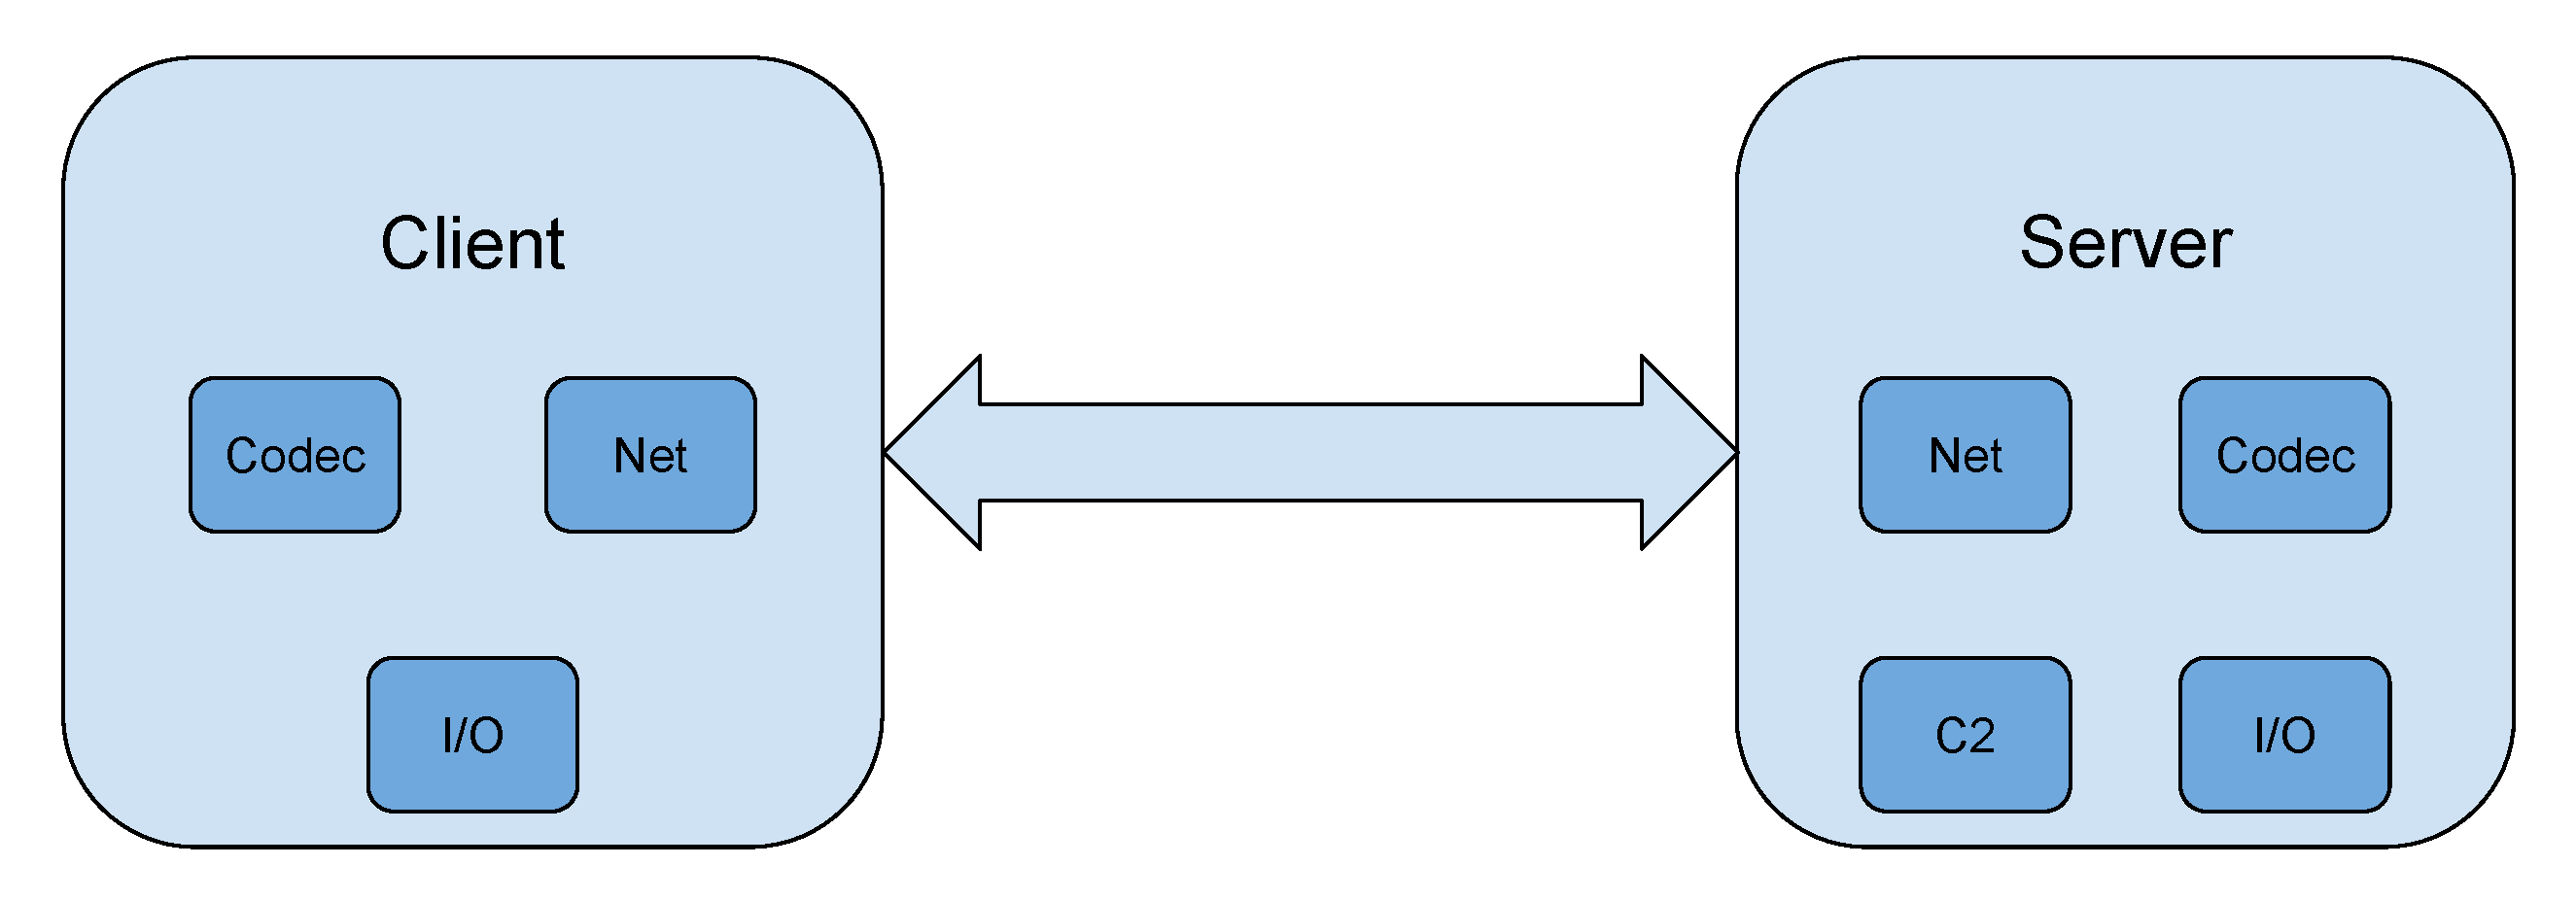
\includegraphics[width=0.5\textwidth]{img/client-server-architecture}
  \caption{Client-Server Model for Covert Communication}
  \label{fig:architecture}
\end{figure}

The server is designed similarly to the client, but features on suplimentary
and critical component, namely the C2 module, which is responsible for command
and control. The control aspect represents user authentication and changing
UID and GID if necessary. The command aspect passes the input received from the
user and attempts to run it as a command, retrieve the output and pass it to the
Codec component.

The way in which our useful data is encoded relies on the options field in the
TCP Header, as outlined in Figure \ref{fig:tcp-header}. The maximum supported
length is 320 bits, or 40 bytes. Most options follow a TLV\footnote{Type, Length, Value}
format. However, routers are known to drop packets with unrecognized options.
Consequently, our solution appears to send a valid TCP option. For this
purpose we use the TCP Alternate Checksum Data option which allows us to
dedicate 37 bytes for useful data, and 3 bytes for TCP options metadata.
This ensures both maximal utilization of the TCP options field and adequate
behavior from intermediary routing equipment.

\begin{figure}
  \centering
  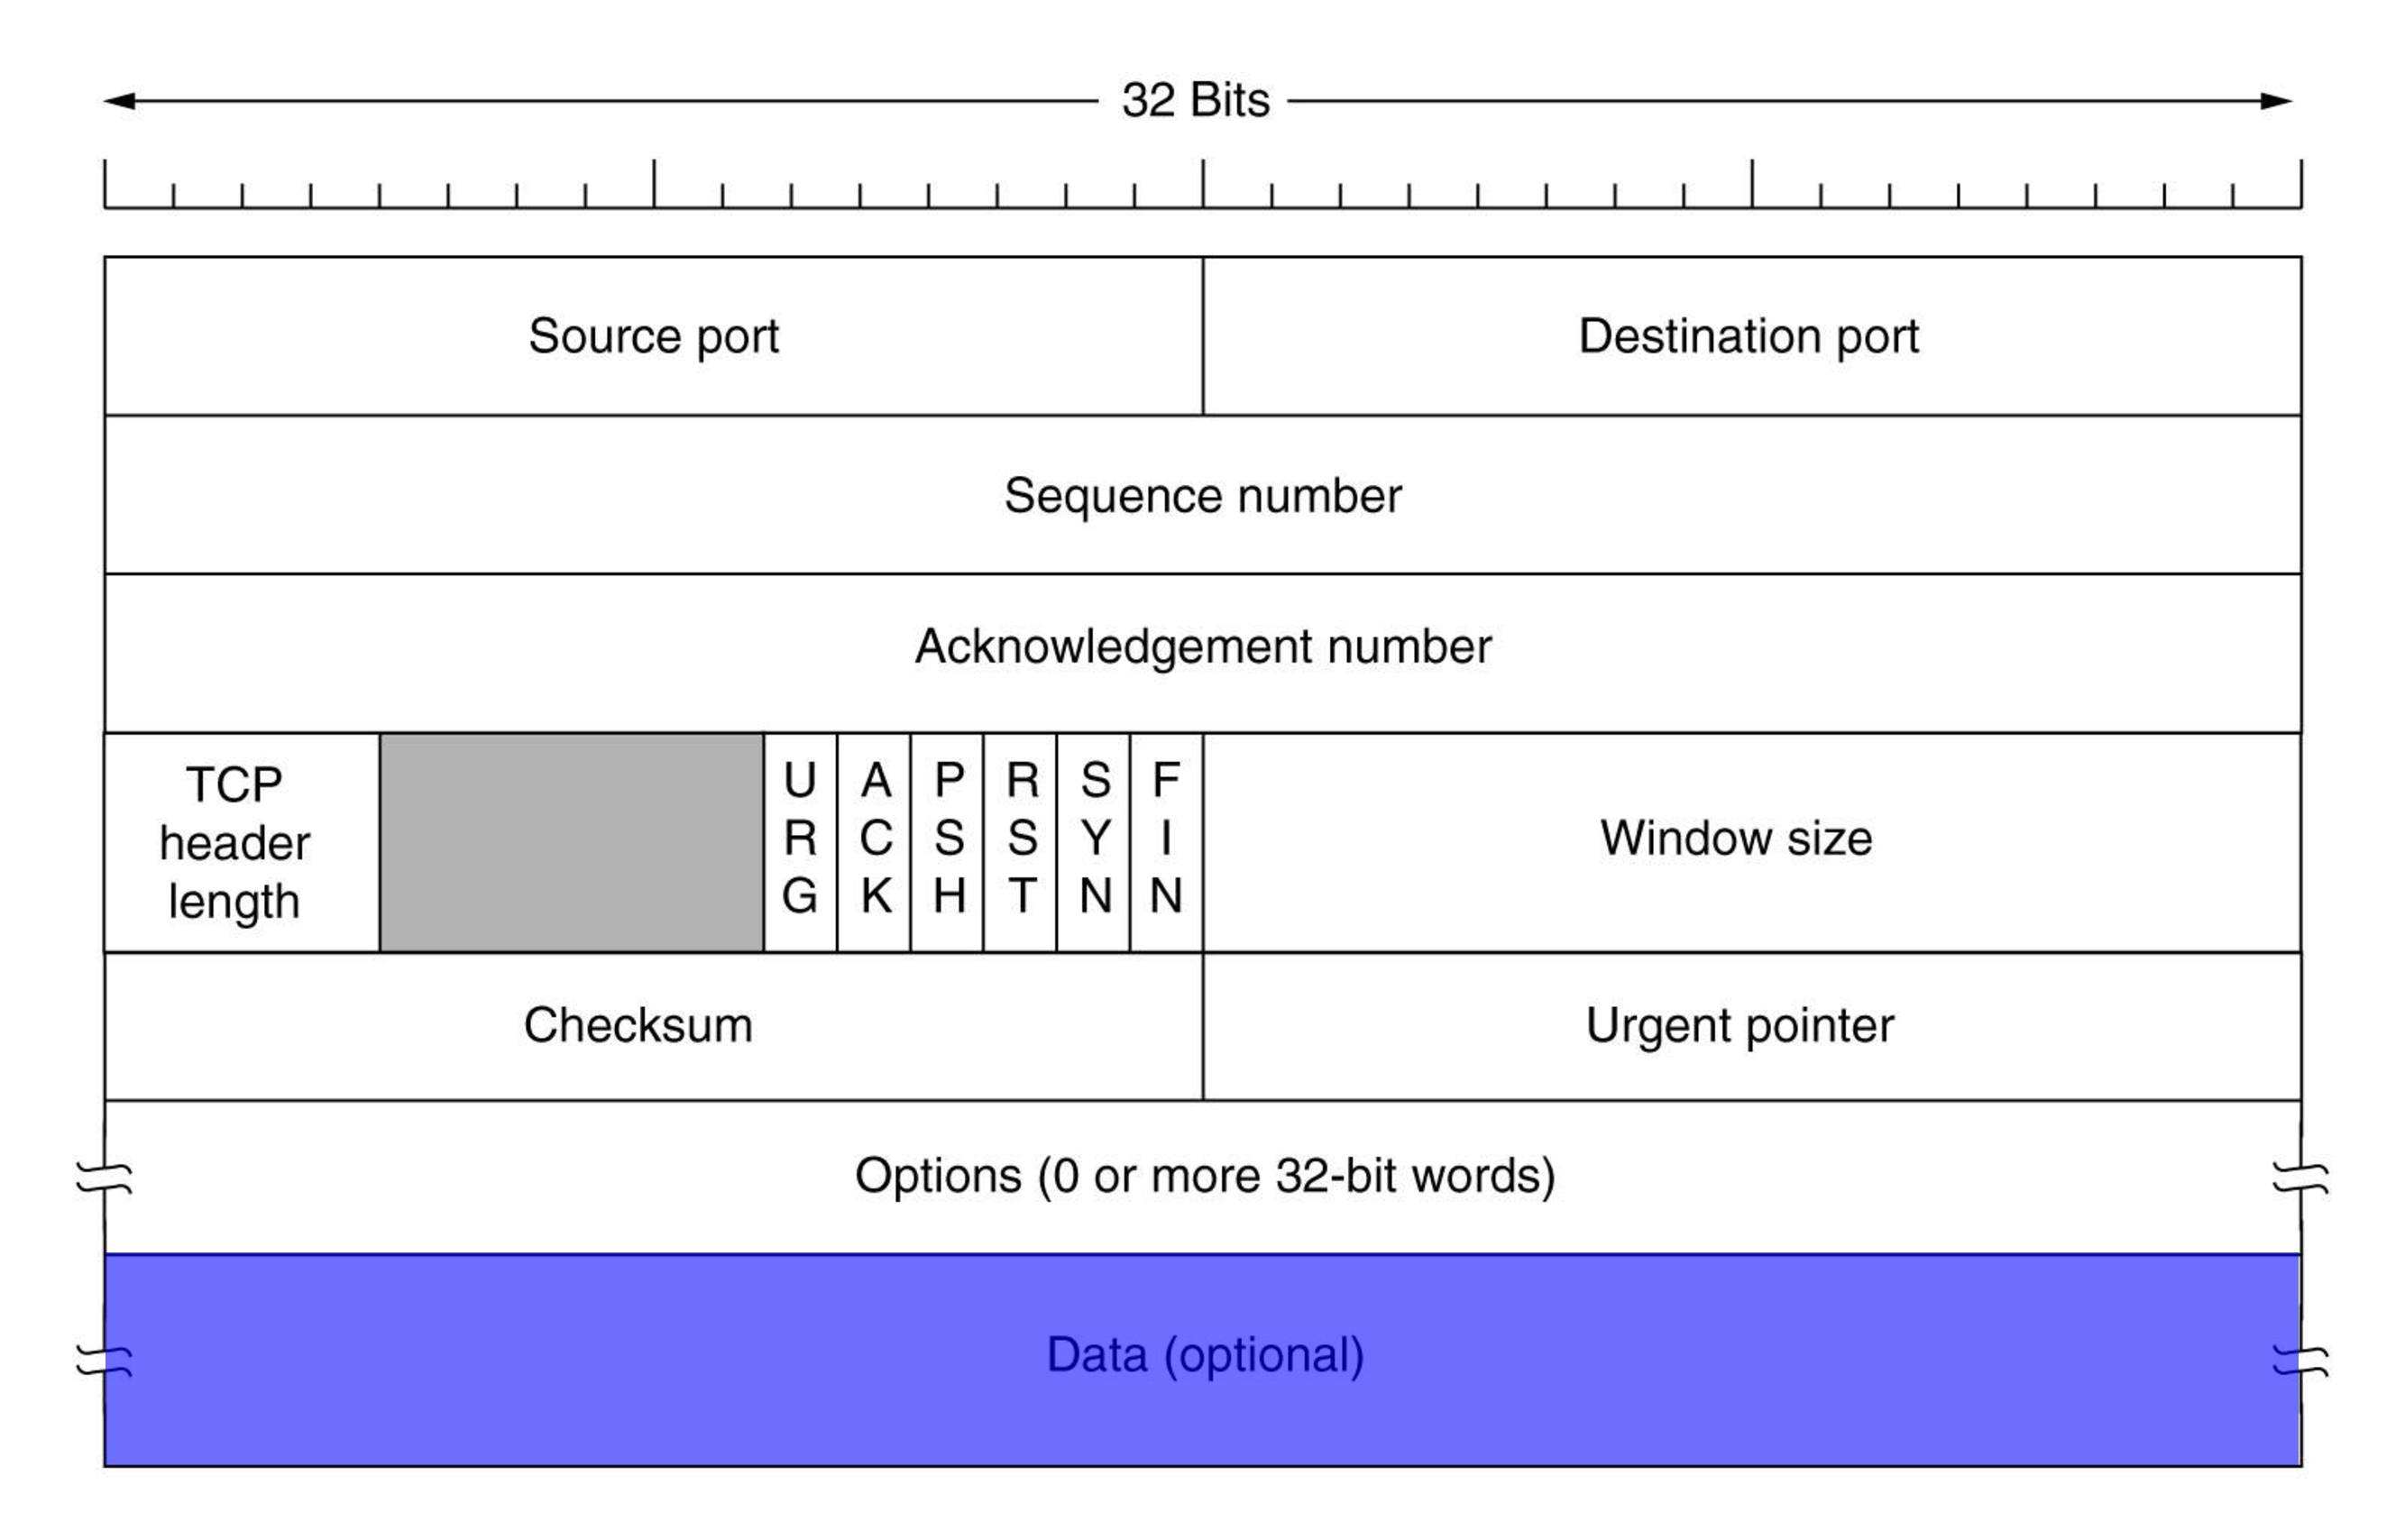
\includegraphics[width=0.5\textwidth]{img/tcp-header}
  \caption{TCP Header}
  \label{fig:tcp-header}
\end{figure}
